\chapter{Theoretical Background}
% \hline
\textit{In Chapter \thechapter, it presents about preliminary knowledge in this project.}
\section{Cosine similarity}

Cosine similarity is a metric that measures the similarity between two vectors of an inner product space. Mathematically, it measures the cosine of the angle between two vectors projected in a multi-dimensional space. The value of cosine of 0 degree is 1, and it is less than 1 for the angles between $(0,\pi)$ radians. In the field of natural language processing, each document is projected in a multi-dimensional space. When using cosine similarity to compare these documents with each other, both vectors are normalized to 1, and the similarity of documents is computed independent of the size of the documents\cite{IJSRSET}.

The formula to find the cosine similarity between two vectors is
\begin{align}
    Similarity(\vec{a},\vec{b}) = cos(\theta)=\frac{\vec{a}\cdot \vec{b}}{||\vec{a}||\hspace{0.1cm}||\vec{b}||}
\end{align}
\section{Transformer}
Transformer is a deep learning architecture showed in figure \ref{fig:transformer} that was introduced in 2017 by Vaswani et al \cite{NIPS2017_3f5ee243}. It builds on the ideas presented in two influential researchs, sequence to sequence \cite{NIPS2014_a14ac55a, DBLP:journals/corr/WuSCLNMKCGMKSJL16} and attention mechanism \cite{luong-etal-2015-effective}, and has become the state-of-the-art architecture for various natural language processing tasks.\\\\
The Transformer Encoder is composed of multiple layers. The first layer is Multi-head Attention, and the second layer is Position-wise Feed-forward network. In the Encoder Self-Attention, Queries, Keys, and Values are all derived from the outputs of the previous Encoder Layer. Both sublayers use a residual connection, inspired by the ResNet architecture \cite{he2016deep}. This additional residual connection is immediately followed by Layer Normalization \cite{ba2016layer}. As a result, the Transformer Encoder produces a vector representation for each position of the input sequence.\\\\
The Transformer Decoder is also a stack of multiple layers. In addition to the two sublayers described in the Encoder, the Decoder includes a third sublayer called the Encoder-Decoder Attention, or Cross-Attention, between these two. In the Encoder-Decoder Attention, Queries are derived from the outputs of the previous Decoder Layer, while the Keys and Values are derived from the Transformer Encoder outputs. In the Decoder Self-Attention, Queries, Keys, and Values are derived from the outputs of the previous Decoder Layer. However, each position in the Decoder can only attend to all positions in the Decoder up to that position, which is called Masked Self-Attention. This Masked Self-Attention preserves the autoregressive property, ensuring that the prediction only depends on those output tokens that have been generated.\\\\
In summary, the transformer model is a powerful and flexible architecture that owes its success to the combination of the sequence to sequence learning approach and the attention mechanism.\\\\ 
\begin{figure}[hbt]
    \centering
    
    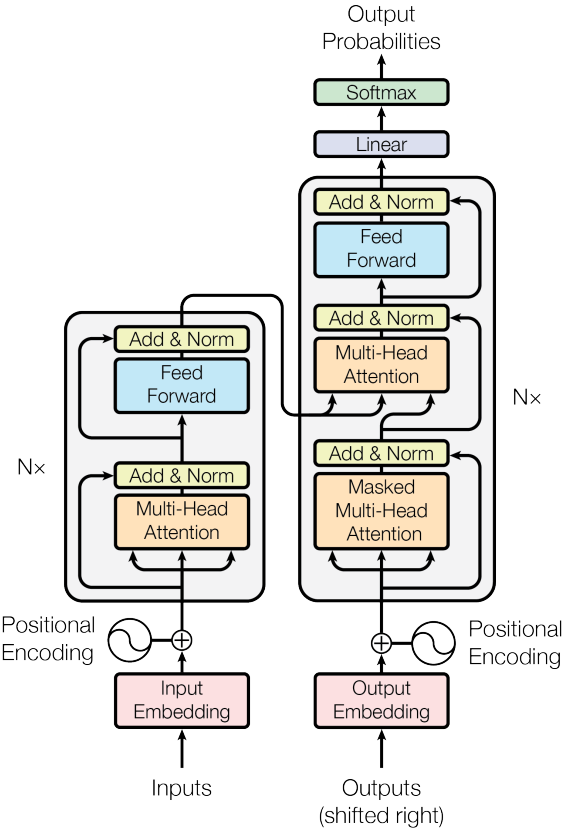
\includegraphics[width=0.6\textwidth]{theoretical-background/image/transformer.png}
    \caption{The architecture of transformers presented in the research paper "Attention is all you need" \cite{NIPS2017_3f5ee243}}
    \label{fig:transformer}
\end{figure}
\textbf{Scaled Dot-Product Attention}: It computes how much each value vector contributes to the output vector, based on the similarity between the query vector Q and the key vector Q. The similarity is measured by the dot product, which is scaled down by the square root of the dimension of the key vector $d_k$. The scaled dot products are then normalized by a softmax function to get the attention weights. The output vector is the weighted sum of the value vectors.
\begin{align}
    Attention (Q,K,V)=softmax(\frac{QK^T}{\sqrt(d_k)})V
\end{align}

\textbf{Multi-head Attention}: It applies the attention function multiple times in parallel, each of them is called a head, using different projections of the query, key and value vectors. This allows the model to capture different aspects of the input and output sequences. The outputs of the multi-head attention are concatenated and projected to get the final output.
\begin{align}
    MultiHead(Q,K,V)= Concat(head_1,...,head_h)W^O\\
    \text{where } head_i=Attention(QW_{i}^Q, KW_{i}^K, VW_{i}^V)
\end{align}

\textbf{Position-wise Feed-forward Networks}: This is a way of transforming the output of the attention layers using a simple neural network that consists of two linear layers with a ReLU activation in between. The network is applied to each position separately and identically, meaning that it does not depend on the order of the sequence. The network has the same input and output dimension as the attention layers, but a larger hidden dimension.
\begin{align}
    FFN(x)=max(0,x\cdot W_1+b_1)\cdot W_2+b_2
\end{align}

\section{Large Language Models}
\begin{figure}[hbt]
    \centering
    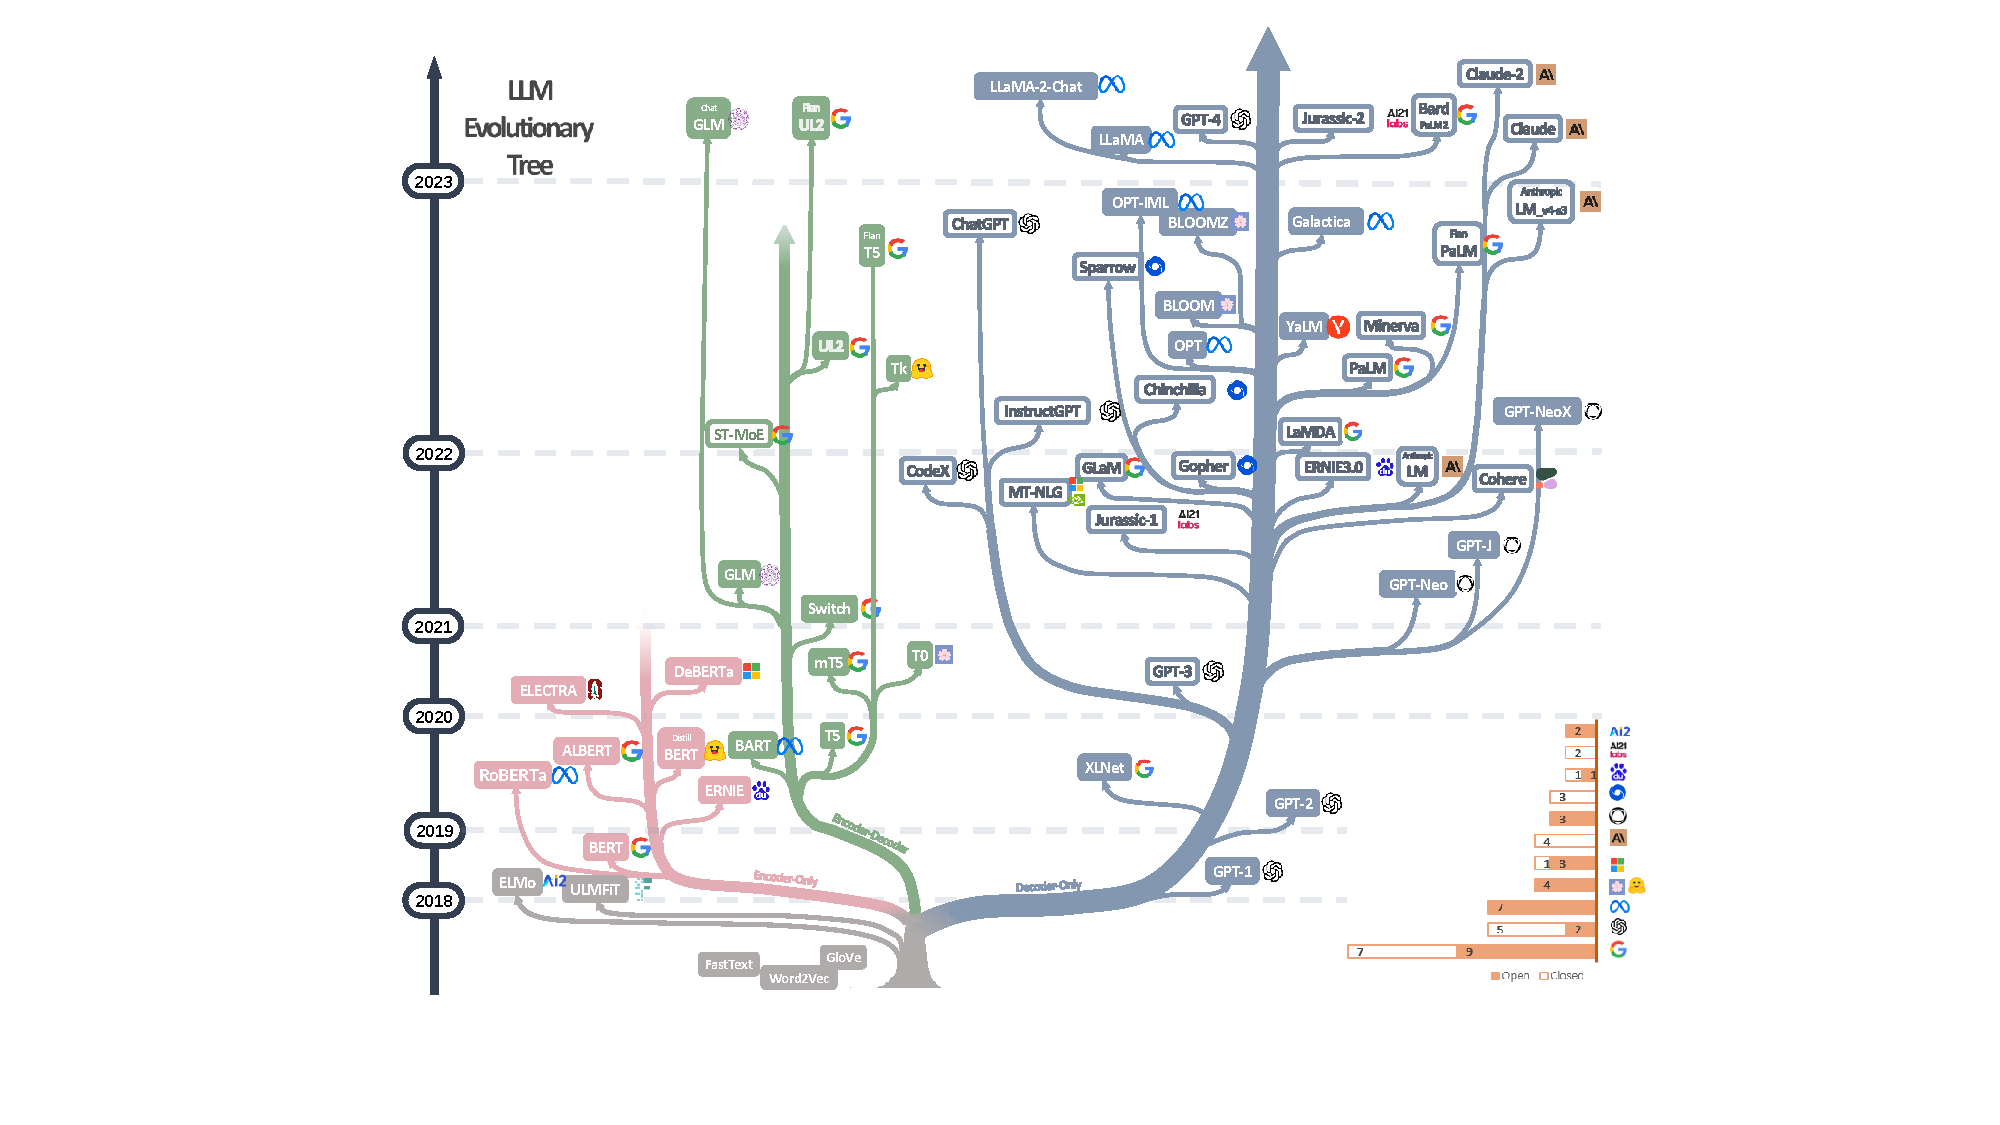
\includegraphics[width=0.95\linewidth]{theoretical-background/image/evo_tree.pdf}
    \caption{The evolutionary tree of modern LLMs traces the development of language models in recent years \cite{yang2023harnessing}}
    \label{fig:evo_tree}
\end{figure}
Large Language Models that are pre-trained on large-scale corpus have demonstrated significant potential in various natural language processing  tasks . Most LLMs are based on the Transformer design, which consists of encoder and decoder modules that are empowered by a self-attention mechanism. Based on their architecture structure, LLMs can be classified into three categories: encoder-only LLMs, encoder-decoder LLMs, and decoder-only LLMs. Figure \ref{fig:evo_tree} summarizes several representative LLMs with different model architectures, model sizes, and open-source availabilities. \\\\
\textbf{Encoder-only LLMs} are a type of Large Language Models that use only the encoder to encode the sentence and understand the relationships between words. These models are typically pre-trained by predicting the mask words in an input sentence using large-scale corpus. To resolve downstream tasks, such as text classification and named entity recognition, an extra prediction head is added to encoder-only LLMs like BERT \cite{devlin-etal-2019-bert}, RoBERTa \cite{liu2019roberta}, ALBERT \cite{lan2019albert}, and ELECTRA \cite{clark2020electra}. These models are most effective for tasks that require understanding the entire sentence.\\\\
\textbf{Encoder-decoder LLMs} adopt both the encoder and decoder module. The encoder module is responsible for encoding the input sentence into a hidden space, and the decoder is used to generate the target output text. The training strategies in encoder-decoder LLMs can be more flexible. Encoder-decoder LLMs are able to directly resolve tasks that generate sentences based on some context, such as summariaztion, translation, and question answering.\\\\
\textbf{Decoder-only LLMs} only adopt the decoder module to generate target output text. These models are trained to predict the next word in a sentence. They can perform downstream tasks with few examples or simple instructions without adding prediction heads or fine-tuning.  \cite{liu2022fewshot}. Many state-of-the-art LLMs follow the decoder-only architecture. Recently Llama-2 \cite{touvron2023llama2}, Alpaca \footnote{https://crfm.stanford.edu/2023/03/13/alpaca.html} and Vicuna \footnote{ https://lmsys.org/blog/2023-03-30-vicuna/} are released as open-source decoder-only LLMs. These models are finetuned based on LLaMA \cite{touvron2023llama} and achieve comparable performance with ChatGPT \cite{ouyang2022training} and GPT-4
\section {Knowledge graph}
Knowledge graphs (KGs) store structured knowledge as a collection of triples $KG = \{(h, r, t) \subseteq E \times R \times E\}$, where E and R respectively denote the set of entities and relations \cite{9416312}. There are four types of existing KGs based on the stored information: Encyclopedic KGs, Commonsense KGs, Domain-specific KGs, and multi-modal KGs.\\\\
\textbf{Encyclopedic KGs}  are the most common type of KGs that store general knowledge about the world. They are usually created by integrating information from various sources such as human experts, encyclopedias, and databases. Wikidata is one of the most popular encyclopedic KGs, which contains a wide range of knowledge extracted from Wikipedia articles \cite{10.1145/2629489}.\\\\
\textbf{Commonsense KGs} are designed to represent knowledge about everyday concepts such as objects and events, as well as their relationships. Unlike encyclopedic knowledge graphs, commonsense knowledge graphs often model tacit knowledge extracted from text, such as the relationship between “Car”, “UsedFor”, and “Drive”. ConceptNet \cite{speer2017conceptnet}, one of the most popular KGs, is a commonsense knowledge graph that contains a wide range of concepts and relations, which can help computers understand the meanings of words people use. \\\\
\textbf{Domain-specific KGs} are created to represent knowledge in a particular domain, such as medicine, biology, or finance. These knowledge graphs are often smaller in size than encyclopedic knowledge graphs, but they are more accurate and reliable. As an instance of a domain-specific knowledge graph, the Unified Medical Language System (UMLS) is a knowledge graph that contains biomedical concepts and their relationships \cite{Bodenreider2004TheUM}.\\\\
\textbf{Multi-modal KGs} are different from conventional knowledge graphs in that they represent facts in multiple modalities such as images, sounds, and videos. For instance, IMGpedia \cite{10.1007/978-3-319-68204-4_8}, MMKG \cite{liu2019mmkg}, and Richpedia \cite{wang2020richpedia} are examples of multi-modal knowledge graphs that incorporate both text and image information into the knowledge graphs. 
\section{Knowledge graph embedding}
Knowledge graph embedding (KGE) aims to represent entities and relations in a knowledge graph as low-dimensional vectors, capturing their semantic relationships. This section focuses on two prominent approaches for KGE: translation models and pretrained language models.
\subsection{Translation models}
Translation models, pioneered by TransE \cite{NIPS2013_1cecc7a7}, are based on the idea of representing relations as translations in the embedding space. For a triple $(h, r, t)$ representing head entity $h$, relation $r$, and tail entity $t$, TransE enforces the following relation:
\begin{align}
\mathbf{h} + \mathbf{r} \approx \mathbf{t}
\end{align}
where $\mathbf{h}$, $\mathbf{r}$, and $\mathbf{t}$ are the embedding vectors of $h$, $r$, and $t$, respectively. This implies that the embedding of the tail entity should be close to the embedding of the head entity translated by the relation vector. TransE utilizes a margin-based ranking loss to encourage correct triples to have lower scores than incorrect ones.
Several extensions to TransE have been proposed to address its limitations in modeling complex relations like one-to-many, many-to-one, and many-to-many. These include TransH \cite{Wang_Zhang_Feng_Chen_2014}, TransR \cite{Lin_Liu_Sun_Liu_Zhu_2015}, and TransD \cite{ji-etal-2015-knowledge}, which introduce relation-specific hyperplanes, projection matrices, and dynamic mapping matrices, respectively, to handle diverse relation patterns.
\subsection{Pretrained language models}
Pretrained Language Models (PLMs), such as BERT \cite{devlin-etal-2019-bert} and RoBERTa \cite{liu2019roberta}, have demonstrated remarkable capabilities in capturing contextualized word representations. Recently, PLMs have been adapted for knowledge graph embedding by treating entities and relations as special tokens within the language model.
KG-BERT \cite{yao2019kg} utilizes BERT for link prediction by transforming it into a masked entity prediction task. Given an incomplete triple $(h, r, ?)$, KG-BERT constructs an input sequence:
\begin{align*}
x_t = \text{\texttt{[CLS]}} h \text{\texttt{[SEP}]} r \text{\texttt{[SEP]}}
\end{align*}
The model then predicts the masked entity by ranking the probability of each entity in the knowledge graph:
\begin{align}
p(t|x_t) = p(\text{\texttt{[CLS]}} = t|x_t;\Phi)
\end{align}
where $\Phi$ represents the model's parameters. KG-BERT is trained using a cross-entropy loss, encouraging the model to assign high probability to the correct tail entity.
This approach effectively leverages the rich semantic information captured by PLMs to learn knowledge graph embeddings. Moreover, it allows for incorporating textual descriptions associated with entities and relations, further enhancing the expressiveness of the embeddings.
By utilizing translation models or pretrained language models, knowledge graph embedding provides a powerful framework for representing and reasoning over knowledge graphs, enabling various downstream tasks such as link prediction, question answering, and recommendation systems.

\section{Direct preference optimization}
Direct preference optimization (DPO) is a learning paradigm that fine-tunes language models to align with user preferences, as introduced in \cite{rafailov2024direct}. Unlike traditional Reinforcement Learning from Human Feedback (RLHF) methods \cite{NIPS2017_d5e2c0ad} that require training a separate reward model and then using reinforcement learning to optimize the policy, DPO directly optimizes the policy to match human preferences using a simple classification objective.
The key insight of DPO is that the optimal policy for a KL-regularized reward maximization objective can be expressed in closed form. This allows us to directly parameterize the policy in a way that implicitly encodes the reward function, bypassing the need for a separate reward model.
Consider a language model policy $\pi_\theta(y|x)$ that generates response $y$ given prompt $x$ and is parameterized by $\theta$. We want to optimize this policy to maximize a reward function $r(x,y)$ while staying close to a reference policy $\pi_{ref}(y|x)$ (usually the initial supervised fine-tuned model). The standard RLHF objective is:
\begin{align}
\max_{\pi_\theta} \mathbb{E}_{x \sim D, y \sim \pi_\theta(y|x)} [ r(x, y)] - \beta D_{KL}[\pi_\theta(y | x) || \pi_{ref}(y | x)]
\end{align}
where $\beta$ controls the strength of the KL penalty.
The optimal solution to this objective has the following form:
\begin{align}
\pi_r(y | x) = \frac{1}{Z(x)} \pi_{ref}(y | x) \exp \left( \frac{1}{\beta} r(x, y) \right)
\end{align}
where $Z(x)$ is the partition function.
DPO leverages this closed-form solution by rearranging it to express the reward function in terms of the optimal policy and the reference policy:
\begin{align}
r(x, y) = \beta \log \frac{\pi_r(y | x)}{\pi_{ref}(y | x)} + \beta \log Z(x)
\end{align}
Substituting this expression for the reward function into a preference model (like the Bradley-Terry model) allows us to express the probability of human preferences directly in terms of the policy and the reference policy. Crucially, the partition function $Z(x)$ cancels out, leaving a tractable objective.
For the Bradley-Terry model, the probability of preferring response $y_w$ over $y_l$ given prompt $x$ is:
\begin{align}
p(y_w \succ y_l | x) = \sigma \left( r(x, y_w) - r(x, y_l) \right)
\end{align}
Substituting the reparameterized reward function and simplifying, we get:
\begin{align}
p(y_w \succ y_l | x) = \sigma \left( \beta \log \frac{\pi_r(y_w | x)}{\pi_{ref}(y_w | x)} - \beta \log \frac{\pi_r(y_l | x)}{\pi_{ref}(y_l | x)} \right)
\end{align}
This leads to the DPO loss function, which is a simple binary cross-entropy loss:
\begin{align}
\mathcal{L}_{DPO} = -\mathbb{E}_{(x, y_w, y_l) \sim D} \log \sigma \left( \beta \left( \log \frac{\pi_\theta(y_w | x)}{\pi_{ref}(y_w | x)} - \log \frac{\pi_\theta(y_l | x)}{\pi_{ref}(y_l | x)} \right) \right)
\end{align}
where $D$ is the dataset of human preference data.
By minimizing this loss, we directly optimize the policy $\pi_\theta$ to match the observed preferences, implicitly learning a reward function that aligns with those preferences. This eliminates the need for a separate reward model and RL, making DPO a simpler and more efficient approach compared to traditional RLHF methods.




% Some possible preliminary knowledge to write in section 2 are:

% Large language models: Explain what are large language models, how they are trained, and what are their advantages and challenges in natural language processing tasks.
% Retrieval-augmented generation: Describe the process of retrieval-augmented generation, which involves retrieving relevant information from a vector database and using it to generate text. Compare this approach with other methods such as fine-tuning or knowledge distillation.
% Knowledge graphs: Introduce the concept of knowledge graphs, which are structured representations of facts and relations among entities. Discuss how knowledge graphs can be used to enhance the knowledge and reasoning abilities of large language models.